
\section{Demonstration Setup}
The \compiler\ demonstration presents the map algebra, the compilation workflow,
and the performance advantages of compiled query processors over alternative
database architectures. In this section we describe the application scenarios
that act as motivating use cases for \compiler, as well as the visualization
tools that convey the technical aspects of query transformations and compiled
executor performance.
Since \compiler\ is suited for applications exhibiting high volume update
streams, in this demonstration, we show \compiler\ processing queries for an
automated trading application making use of NASDAQ TotalView order book
data~\cite{totalview-url}, and emulating a combined data warehouse loading and
analysis application for TPC-H data. 

\smallskip
\noindent\textbf{Processing order books in equities trading.}
Order books provide a superior view of the market microstructure for use in
trading algorithms. The bid order book consists of prices and volumes at which
investors are willing to buy equities, and correspondingly the ask order book
indicates investors' selling orders.
\comment{
Exchanges execute trades by matching the tops of the bid and ask order
books.
}
Investors continually add, modify or withdraw limit orders, thus we regard order
books as relations subject to high volumes of order deltas. Note order books do
not grow unboundedly in practice, but cannot be expressed by windows given
arbitrary input deltas. We present a few queries in the automated trading
application, first a volume-weighted average price (VWAP) query which computes
the average price-volume product of orders making up a given fraction of volume
in the bid and ask order books. One example usage of the VWAP metric is for a
static order book imbalance (SOBI) trading strategy, which detects trade price
movements based on whether there is greater activity in the bids or asks order
book. The final query detects strategies being employed by market makers through
the order book, where market makers often submit orders to entice buyers or
sellers into the market to aid in balancing their position.

\smallskip
\noindent\textbf{Data warehouse loading.}
Loading large data warehouses is a computation-intensive process, hence most
data warehouse loading is performed offline. While commercial warehouse loaders use
highly tuned code for aggregation, incoming data is often the result of costly,
inefficient data integration queries, which often blow up data sizes to cause
inefficient loading. Compiling data integration and aggregation queries together
yields efficient code for loading the warehouse and may avoid the
materialization of large intermediate results.
We use \compiler\ to jointly process loading a warehouse from an OLTP database,
and an aggregation query on the warehouse. We emulate the data integration step
by using a data cleaning query to convert a TPC-H dataset into a star schema from
the Star Schema Benchmark (SSB)~\cite{poneil-ssb:07}. We then evaluate query 4.1
from SSB on the transformed TPC-H dataset.

\smallskip
\noindent\textbf{Interactive demonstration.}
An integral part of this demo is to support interaction with conference
attendees, thus in addition to providing canned queries implementing these
applications, we allow attendees to directly pose their own queries on
the TotalView and TPC-H datasets.



\subsection{Query compilation and code generation}

\begin{figure}[tb]
\begin{center}
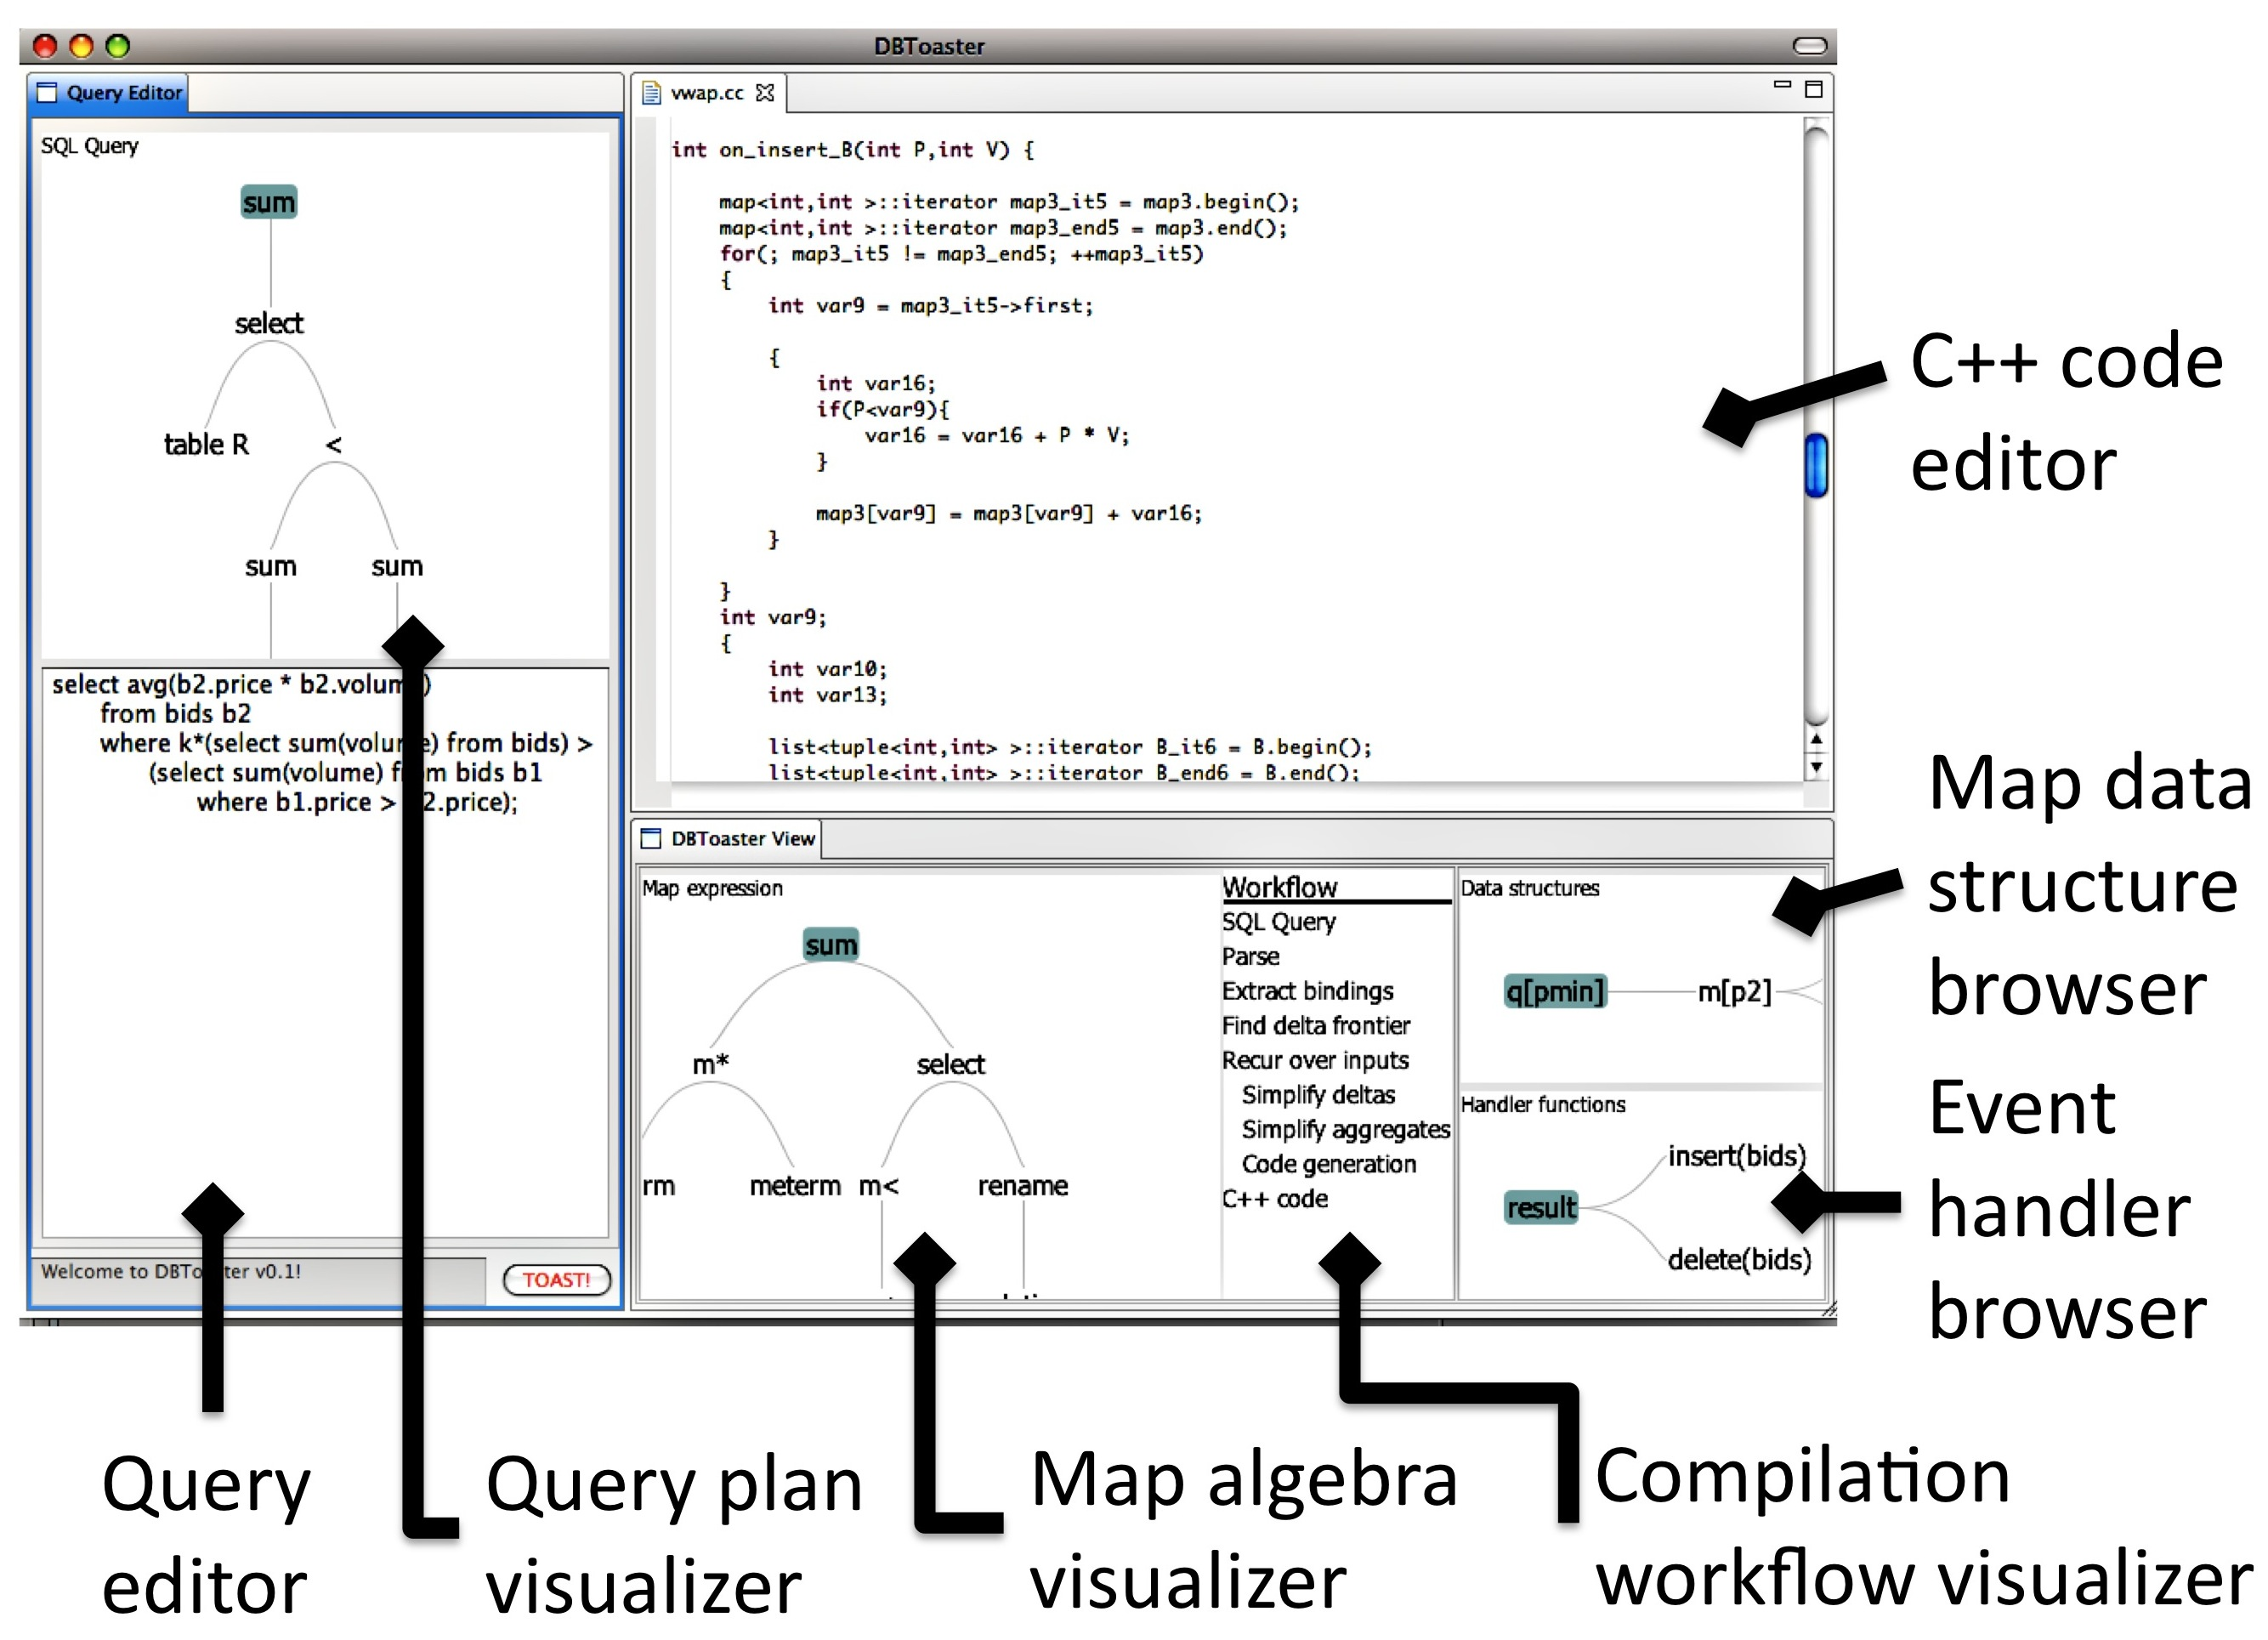
\includegraphics[scale=0.088]{figures/dbt-gui}
\end{center}

\vspace{-4mm}

\caption{\compiler\ compilation process visualization, displaying map algebra
transformations, generated code, and internal views maintained.}
\label{fig:compilegui}

\vspace{-2mm}
\end{figure}

The first of our two visualization tools, Figure.~\ref{fig:compilegui}, conveys
the compilation process to demo attendees. This tool visually displays a standard
relational query plan, and illustrates the compiler workflow in a step-by-step
fashion, including map algebra simplifications and the maps instantiated during
compilation. We place particular emphasis on the recursive nature of our
compilation, demonstrating compilation of deltas on the queries corresponding to
our map data structures. At this point query compilation is complete, and we use
a pair of browser windows listing both the maps and the event handling functions
generated to aid in discussions with attendees. We also use a debugging tool to
provide step-by-step tracing of map maintenance when processing a delta.
\comment{ Depending on the
demonstration progress, we may additionally include an example of a
JIT-compilation of the example query to demonstrate the potential for a limited
degree of adaptivity during query execution.
}

\begin{figure}[tb]
\begin{center}
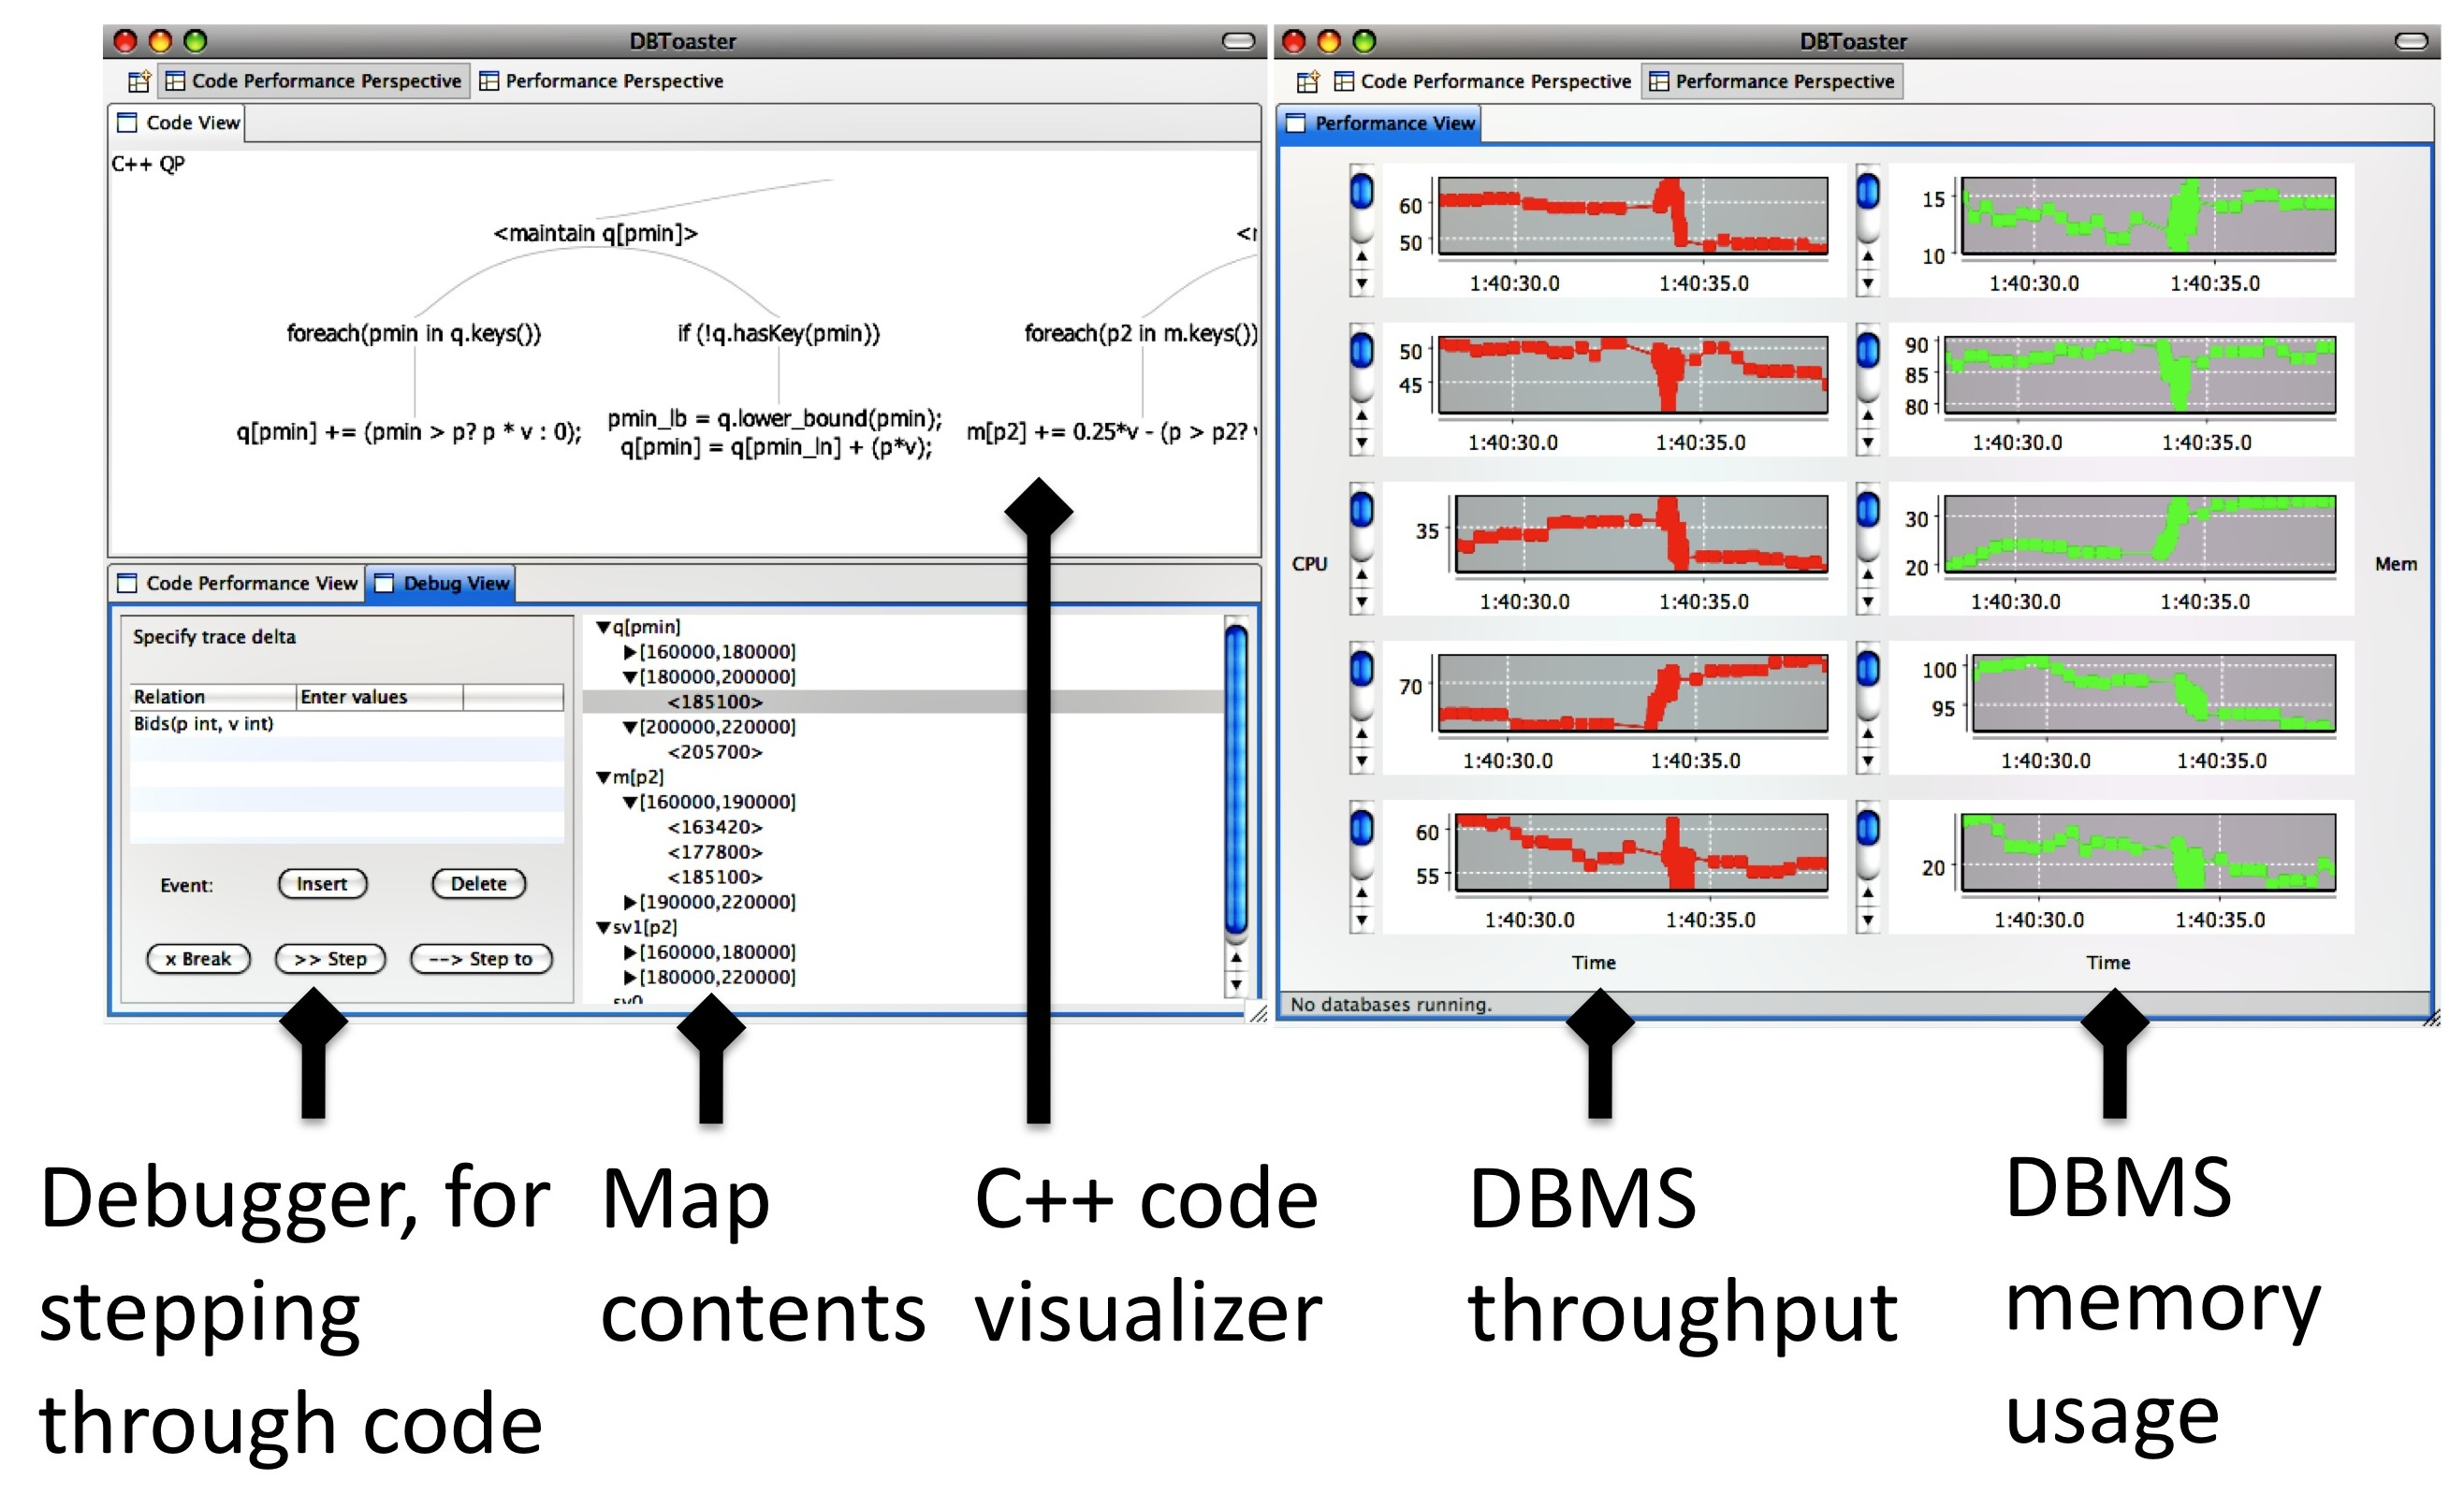
\includegraphics[scale=0.088]{figures/dbt-gui2}
\end{center}

\vspace{-4mm}

\caption{\compiler\ debugger supporting stepping and tracing query processing and
map maintenance, and performance visualizer for comparing against alternative
databases in the DBMS bakeoff.}
\label{fig:debugperfgui}

\vspace{-2mm}
\end{figure}

\vspace{10mm}

\subsection{\compiler\ vs. DBMS* Bakeoff}
This demo also presents \compiler's competitiveness with a variety of database
tools, by performing a DBMS bakeoff. Our comparison points are PostgreSQL, a pure
Java main-memory DBMS (HSQLDB~\cite{hsqldb-url}), a commercial DBMS 'A', the
Stanford STREAM engine~\cite{motwani-cidr:03}, and a commerical stream processor
'B'. We have a visualization tool (Figure.~\ref{fig:debugperfgui}) to show the
performance achieved by the each database system including tuple throughput,
memory usage and cache performance. We also present detailed profiling of
\compiler's compiled code breaking down its overheads for each map, the binary
size, and finally the compile time including both the C++ generation and the
subsequent compilation to a native binary. To provide an entertaining audience
experience, we run an audience challenge to find queries both yielding the
greatest performance over the other database engines in the bakeoff, as well as
queries that illustrate the poorest performance. Attendees will be provided with
two laptops at the demonstration booth to experiment with queries, and encourage
participation by displaying a leaderboard of the running results.

